% !TeX root = main.tex
\chapter{随机变量与分布函数}
\section{随机变量及其分布
}
随机变量是一个事件到实数(轴上的Borel集)的映射,目的在于数值化样本点。之所以掷骰子点数的期望看起来不自然,
是因为他依赖于随机变量对事件的映射。随机变量还允许我们对变量进行数学运算。\[
    \xi \sim N(0,1) \iff \xi+1 \sim N(1,1)
\]

分布是随机变量的概率性质。

分布函数是随机变量取值小于等于某个特定值的概率。在离散型随机变量里,分布列是随机变量取特定值的结果。在连续型随机变量里,
概率密度函数是分布函数的导数。二者都把概率刻画成一定的直观测度,但截然不同。不可能通过趋于无穷的分布列逼近概率密度函数,
因为此时分布列必然所有元素都趋于0。但分布函数是可以由离散向连续逼近的。

% TODO: 增加二项分布逼近超几何分布

\subsection{离散型随机变量}
% 伯努利试验
% 二项分布的简单介绍
% 几何分布的无记忆性
\paragraph{几何分布} 在成功的概率为\(p\) 的伯努利试验中,若以第\(\zeta\)
记第一次成功出现时的试验次数为随机变量\(\zeta\),则\(\zeta\) 服从几何分布:
\[
    \P{\zeta=k} = (1-p)^{k-1} p, \quad k=1,2,\ldots
\]

% 由几何分布推导帕斯卡分布
\paragraph{帕斯卡分布} 在成功的概率为\(p\) 的伯努利试验中,若以第\(\zeta\) 记第\(r\)
次成功出现时的试验次数为随机变量\(\zeta\),则\(\zeta\) 服从帕斯卡分布:
\[
    \P{\zeta=k} = \binom{k-1}{r-1} p^r
    (1-p)^{k-r}, \quad k=r,r+1,\ldots
\]

% TODO:负二项分布?有什么用?

帕斯卡分布与几何分布有以下关系:若以\(\nu_{i}\) 记第\(i-1\) 次成功后第一次试验算起至第\(i\)
次成功为止进行的的试验次数,则\(\nu_{i}\) 相互独立、服从几何分布,且:
\[
    \zeta = \nu_{1} + \nu_{2} + \cdots + \nu_{r}
\]

我们实际上可以从此直接推导出帕斯卡分布的概率分布:
由\(\zeta = \nu_{1} + \nu_{2} + \cdots + \nu_{r}\) 有:
\begin{align*}
    \P{\zeta=k} &=
    \sum_{\substack{i_{1}+i_{2}+\dots +i_{r}=k
    \\ i_{1},i_{2},\ldots,i_{r}\geq 1}} \P{\nu_{1}=i_{1},
    \nu_{2}=i_{2}, \ldots, \nu_{r}=i_{r}} \\
    &=\sum_{\substack{i_{1}+i_{2}+\dots +i_{r}=k
    \\ i_{1},i_{2},\ldots,i_{r}\geq 1}} P\left\{
    \nu_{1}=i_{1}\right\} \P{ \nu_{2}=i_{2} }
    \cdots \P{ \nu_{r}=i_{r} } \\
    &= \sum_{\substack{i_{1}+i_{2}+\dots +i_{r}=k
    \\ i_{1},i_{2},\ldots,i_{r}\geq 1}} p(1-p)^{i_{1}-1}
    \cdot p(1-p)^{i_{2}-1} \cdots p(1-p)^{i_{r}-1} \\
    &= \sum_{\substack{i_{1}+i_{2}+\dots +i_{r}=k
    \\ i_{1},i_{2},\ldots,i_{r}\geq 1}} p^{r} (1-p)^{k-r} \\
    &= \binom{k-1}{r-1} p^{r} (1-p)^{k-r}
\end{align*}

概率论就是这样,事情很容易变得(看起来)过分复杂\UseVerb{sad}。

\subsection{连续型随机变量}
% 伯努利试验推导泊松分布(直观+公式)
% 指数分布的直观推导与无记忆性
% Erlang分布的推导和指数分布的推导过来
% TODO: 正态分布切片还是正态分布?
% TODO: P130计算机字长造成的误差是什么分布?不是对数分布?
% TODO: P137当时间紧迫我们应该求稳还是冒险
考虑在一小时内把时间划分为\(n\) 份进行伯努利试验,并期望得到\(\lambda\)次试验结果。那么随着\(n
\to \infty\),得到结果次数\(k\) 服从的二项分布将逐渐逼近泊松分布。这就是泊松分布的意义。

\paragraph{Erlang分布} Erlang分布是帕斯卡分布的连续型版本。若\(\xi(t)\)
是参数为\(\lambda t\) 的泊松过程,以\(W_{t}\) 记第\(r\) 个跳跃发生的时刻。

Erlang分布和指数分布的关系与几何分布和帕斯卡分布的关系类似,记\(\tau_{r}\) 是泊松过程第\(r\)
个跳跃的发生间隔,则\(\tau_{r}\) 相互独立且满足指数分布,且:
\[
    W_{t} = \tau_{1} + \tau_{2} + \cdots + \tau_{r}
\]

同样的,我们可以从此式推导出Erlang分布的概率分布:
\begin{align*}
    \P{W_{r}<t} &= \P{\tau_{1}+\tau_{2}+\cdots+\tau_{r}<t} \\
    &= \int\limits_{\substack{x_{1}+x_{2}+\dots +x_{r}<t
    \\ x_{i}>0, i=1,2,\ldots,r}} p(x_{1}) p(x_{2}) \cdots p(x_{r})
    \d{x}_{1} \d{x}_{2} \cdots \d{x}_{r} \\
    &=\int_{0}^{t} \lambda \e^{-\lambda x_{1}} \d{x_{1}}
    \int_{0}^{t-x_{1}} \lambda \e^{-\lambda x_{2}} \d{x_{2}} \cdots
    \int_{0}^{t-x_{1}-\cdots-x_{r-1}} \lambda \e^{-\lambda
    x_{r}} \d{x_{r}} \\
\end{align*}

记:
\begin{align*}
    I_{0}(t) &= 1\\
    I_{r+1}(t) &= \int_{0}^{t} I_{r}(t-x) \lambda \e^{-\lambda x} \d{x}
    \end{align*}
则:\(\P{W_{r}<t} = I_{r}(t)\)

我们用Laplace变换来求解这个递推积分。
记\(g(x) = \lambda \e^{-\lambda x} \) 。
注意到:
\[
    \L{I_{0}(t)} = \L{1} = \frac{1}{s} \\
\]
\begin{align*}
    \L{I_{r+1}(t)} &= \L{(g * I_{r})(t)} \\
    &= \L{g(t)} \cdot \L{I_{r}(t)} \\
    &= \frac{\lambda}{(s+\lambda)} \L{I_{r}(t)}\\
\end{align*}
从而:\[
    \L{I_{r}(t)} = \frac{\lambda^{r}}{s(s+\lambda)^{r}} \\
\]
Erlang分布的概率密度函数为:
\begin{align*}
    p(t) = I_{r}'(t) &= \invL{\L{I_{r}'(t)}} \\
    &= \invL{s\L{I_{r}(t)} - I_{r}(0)} \\
    &= \invL{\frac{\lambda^{r}}{(s+\lambda)^{r}}} \\
    &= \frac{\lambda^{r}}{(r-1)!} \lambda \e^{-\lambda t} \\
\end{align*}

由上我们看到,独立随机变量的和的密度函数就是两随机变量密度函数的卷积。\footnote{其实如果我要没这么猴急,
下一节我就能学到这点\UseVerb{sad}}

\section{随机向量、随机变量的独立性}
\subsection{随机向量及其分布}
% 随机向量分布函数定义
% 随机向量计算区域概率和非负性说明
% 病态随机向量
联合分布不能由边际分布唯一确定
\subsection{条件分布}
\[
    p(y\mid x)=\frac{p(x,y)}{p(x)} \\
\]
二元正态分布的条件分布、边际分布都是正态分布。
% 正态分布标准分解
\subsection{随机变量的独立性}
随机变量的独立性为我们提供了拆括号的可行性:
\begin{align*}
    \P{\xi_{1} \leq x_{1}, \xi_{2} \leq x_{2}, \dots ,
    \xi_{n} \leq x_{n}} &=
    \P{\xi_{1} \leq x_{1}} \cdot
    \P{\xi_{2} \leq x_{2}} \cdots
    \P{\xi_{n} \leq x_{n}}\\
    \P{\bm{\xi} \in A, \bm{\eta} \in B} &=
    \P{\bm{\xi} \in A} \cdot
    \P{\bm{\eta} \in B} \\
    p(x_{1},x_{2},\ldots,x_{n}) &= p(x_{1}) \cdot p(x_{2})
    \cdots p(x_{n}) \quad (a. e.)
\end{align*}
二元正态分布两变量相互独立当且仅当\(\rho=0\)

两组具有相同分布的随机变量可以是相互独立的,也可以不是相互独立的。
% TODO: Add a.e. support
% TODO: Add deduction of Normal distribution

\section{随机变量的函数及其分布}

\paragraph{对数正态分布}
% TODO: The relationship Chi-square distribution and Chi-Square Test
若\(\xi\sim N(\mu,\sigma^{2})\), 则\(\eta=\e^{\xi} \) 服从对数正态分布:
\[
    q(y) = \frac{1}{\sqrt{2\pi}\sigma y}
    \e^{-\frac{(x-\mu)^{2}}{2\sigma^{2}}}\quad y>0
\]
对数正态分布在对自然现象的描述中非常重要。许多自然增长过程是由许多小的百分比变化累积驱动的,
这些变化在以对数尺度为基准时是可加的。在适当的正则条件下,这些累积变化的结果分布将越来越接近对数正态分布。
例如,矿物中稀有元素的浓度符合对数正态分布。以下是地壳中元素浓度的\textbf{对数}分布图,近似满足正态分布。
\begin{figure}[H]
    \centering
    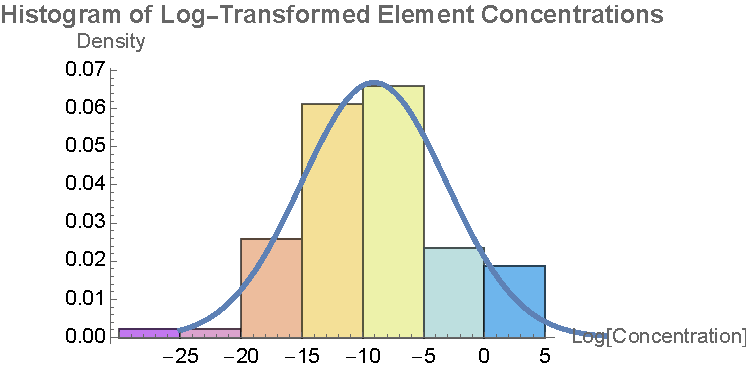
\includegraphics[width=0.7\textwidth]{resources/element_concentration.pdf}
    \caption{地壳中元素浓度的对数分布图}
    \label{fig:lognormal}
\end{figure}\footnote{使用Mathematica绘制,源代码可见
\href{https://github.com/Sazzzzzz/MathNotes/blob/main/code_demos/log_normal_dist_demo.nb}{\texttt{MathNotes/code_demos/log_normal_dist_demo.nb}}}
% TODO: Fix the graph
更多对数正态分布的应用可见
\href{https://en.wikipedia.org/wiki/Log-normal_distribution#Occurrence_and_applications}{Wikipedia}